
\chapter{Propuesta de Arquitectura y Modelo de Base de Datos}\label{chapter:implementation}

\subsection{Arquitectura propuesta}
\label{chapter:implementation}

% cita aqui
\textbf{Model-View-ViewModel (MVVM)}  es un patrón de arquitectura que surgió como alternativa a los patrones $Model$ $View$ $Controller$ y $Model$ $View$ $Presenter$ \brackcite{mvvm} que tiene el objetivo para llevar a cabo la separación del apartado de la interfaz de usuario ($View$) de la parte lógica ($Model$). Esto lo hace con el objetivo de que el aspecto visual sea completamente independiente.

El recurso de $ViewModel$, por su lado, destaca como el componente que se encargará de servir como puente entre la interacción de la Vista ($View$) y el Modelo ($Model$).

\begin{itemize}
\item \textbf{View}: este componente representa la interfaz de usuario y se conforma de un grupo de $Pages$\footnote{En $Flutter$ un $Page$ es una pantalla que es visible en un momento dado.} que actúan como interfaz de los servicios que ofrece la aplicación. Cada $Page$ está compuesta por $Widgets$\footnote{Los $widgets$ componentes utilizados para crear la interfaz de usuario de la aplicación .} con los que el usuario interactúa. 
\item \textbf{Model}: este componente representa la lógica de la aplicación y se conforma por los componentes que refieren a los servicios de comunicación con el servidor, almacenamiento interno de datos y comunicación con otro dispositivo.
\item \textbf{ViewModel}: este componente está conformado por un grupo de interfaces que establecen una comunicación entre la Vista y el Modelo.

\end{itemize}




Los autores consideraron que el patrón $MVVM$ aportaba el beneficio de permitir crear pruebas unitarias para el $ViewModel$ y el $Model$ sin que fuera necesario el uso del $View$. También aportaba el beneficio de poder trabajar en el diseño y desarrollo de la aplicación de manera independiente y simultánea.


\subsection{Modelo de Datos}

Para persistir los datos necesarios en el cumplimiento de los requerimientos de la aplicación, es fundamental el empleo de una base de datos. Con esto en mente, se consideró el uso de una $base$ $de$ $datos$ $relacional$, la cual se elaboró teniendo en cuenta el buen diseño del modelo de datos para una ampliación del mismo de manera sencilla  (ver Figura $3.1$). El modelo diseñado consta de \textbf{quince entidades} las cuales son descritas a continuación:

\textbf{Allergies}, \textbf{Drug}, \textbf{Vaccines} y \textbf{Disease} son las tablas que contienen las definiciones por defecto de las alergias, los medicamentos, las vacunas y las enfermedades respectivamente:

\begin{itemize}
\item	$id$ ($PK$\footnote{Llave primaria, $Primary$  $Key$ por sus siglas en inglés.} ): Valor entero que identifica de forma única cada una de las filas de estas tablas.
\item	$name$: Texto utilizado para nombrar una alergia, un medicamento, una vacuna o una enfermedad dependiendo del caso.

\end{itemize}

\textbf{Pets} es la tabla que contiene la información básica de las mascotas:

\begin{itemize}
\item	$idPet$ ($PK$): Valor entero que identifica de forma única una fila de esta tabla y por ende a una mascota.
\item	$idPerson$: Texto utilizado para identificar de forma única al dueño de la mascota.
\item	$name$: Texto utilizado para almacenar el nombre de una mascota.
\item	$date$: Texto utilizado para almacenar la fecha de nacimiento de una mascota.
\item	$species$: Texto que contiene la especie a la que pertenece una mascota.
\item	$race$: Texto que contiene la raza a la que pertenece una mascota.
\item	$gender$: Texto que contiene el género de una mascota.
\item	$bloodType$: Texto que representa el tipo de sangre de una mascota.
\item	$own$ : Valor entero utilizado para identificar si una mascota es propia o no.
\item	$state$: Texto utilizado por la base de datos para identificar en cual estado se encuentra una mascota. Puede tener los siguientes valores:
\begin{itemize}
\item	$empty$: significa que una mascota fue creada pero sus datos aún no se han llenado.
\item	$delete$: significa que la mascota ha sido eliminada pero aún no se ha notificado al servidor.
\item	$waiting$: significa que se han llenado los campos de la mascota, pero aún no se ha notificado al servidor.
\item	$synchro$: significa que ya se ha notificado al servidor los cambios referentes a la mascota.
\end{itemize}
\end{itemize}

\textbf{MedicalVisit} es la tabla que contiene la información de las visitas médicas:

\begin{itemize}
\item	$uid$ ($PK$): Texto que identifica de forma única una fila de esta tabla.
\item	$idPet$ ($FK$\footnote{Llave foránea, $Foreign$ $Key$ por sus siglas en inglés.} ): Valor entero que identifica de forma única una fila de la tabla $Pets$.
\item	$idPerson$: Texto que identifica de forma única a la persona que insertó una visita médica en la aplicación.
\item	$date$: Texto utilizado para almacenar la fecha de una visita médica.
\item	$place$: Texto que representa el lugar en el que se realizó una visita médica.
\item	$doctor$: Texto que contiene el nombre del médico o especialista que realizo una visita médica.
\item	$notes$: Texto utilizado para almacenar notas extras sobre una visita médica.
\item	$state$\footnote{Puede ser waiting o synchro.} : Texto utilizado por la base de datos para identificar en cual estado se encuentra una visita médica.
\end{itemize}

\textbf{LabTests} es la tabla que se utiliza para almacenar las pruebas de laboratorio:

\begin{itemize}
\item	$uid$ ($PK$): Texto que identifica de forma única una fila de esta tabla.
\item	$idPet$ ($FK$): Valor entero que identifica de forma única una fila de la tabla $Pets$.
\item	$idPerson$: Texto que identifica de forma única a la persona que insertó una prueba de laboratorio en la aplicación.
\item	$date$: Texto utilizado para almacenar la fecha en la que se realizó una prueba de laboratorio.
\item	$place$: Texto en el que se guarda el lugar en el cual se realizó una prueba de laboratorio.
\item	$doctor$: Texto que almacena el nombre del especialista que realizó una prueba de laboratorio.
\item	$test$: Texto que identifica el test realizado en una prueba de laboratorio.
\item	$result$: Texto que almacena el resultado de una prueba de laboratorio.
\item	$normal$ : Valor entero que representa si una prueba de laboratorio fue normal o no.
\item	$notes$: Texto utilizado para almacenar notas extras sobre una prueba de laboratorio.
\item	$state$: Texto utilizado por la base de datos para identificar en cual estado se encuentra una prueba de laboratorio.
\end{itemize}

\textbf{Prescription} es la tabla que almacena las prescripciones:

\begin{itemize}
\item	$uid$ ($PK$): Texto que identifica de forma única una fila de esta tabla.
\item	$idPet$ ($FK$): Valor entero que identifica de forma única una fila de la tabla $Pets$.
\item	$idMedicament$ ($FK$): Valor entero que identifica de forma única una fila de la tabla $Drug$.
\item	$idPerson$: Texto que identifica de forma única a la persona que insertó una prescripción en la aplicación.
\item	$dose$: Texto que representa la dosis del medicamento recetado en una prescripción.
\item	$date$: Texto que almacena la fecha en la que se realizó una prescripción.
\item	$place$: Texto que representa el lugar donde se realizó una prescripción.
\item	$doctor$: Texto que contiene el nombre del especialista que realizó una prescripción.
\item	$notes$: Texto utilizado para almacenar notas extras sobre una prescripción.
\item	$state$: Texto utilizado por la base de datos para identificar en cual estado se encuentra una prescripción.

\end{itemize}

\textbf{Allergy} es la tabla que almacena las alergias de las mascotas.
\begin{itemize}


\item	$uid$ ($PK$): Texto que identifica de forma única una fila de esta tabla.
\item	$idPet$ ($FK$): Valor entero que identifica de forma única una fila de la tabla $Pets$.
\item	$idAllergy$ ($FK$): Valor entero que identifica de forma única una fila de la tabla $Allergies$.
\item	$idPerson$: Texto que identifica de forma única a la persona que insertó una alergia en la aplicación.
\item	$date$: Texto utilizado para almacenar la fecha en la que se detectó una alergia.
\item	$notes$: Texto utilizado para almacenar notas extras sobre la detección de una alergia.
\item	$state$: Texto utilizado por la base de datos para identificar en cual estado se encuentra una alergia.
\end{itemize}


\textbf{Condition} es la tabla para almacenar las condiciones o enfermedades que tienen las mascotas:

\begin{itemize}
\item	$uid$ ($PK$): Texto que identifica de forma única una fila de esta tabla.
\item	$idPet$ ($FK$): Valor entero que identifica de forma única una fila de la tabla $Pets$.
\item	$idDisease$ ($FK$): Valor entero que identifica de forma única una fila de la tabla $Disease$.
\item	$idPerson$: Texto que identifica de forma única a la persona que insertó una condición en la aplicación.
\item	$name$: Texto utilizado para guardar el nombre del diagnóstico de una condición.
\item	$date$: Texto utilizado para almacenar la fecha en la que se diagnosticó una condición.
\item	$place$: Texto en el que se guarda el lugar en el cual se diagnosticó una condición.
\item	$doctor$: Texto que almacena el nombre del especialista que diagnosticó una condición.
\item	$notes$: Texto utilizado para almacenar notas extras sobre el diagnóstico de una condición.
\item	$state$: Texto utilizado por la base de datos para identificar en cual estado se encuentra el diagnóstico de una condición.
\end{itemize}

\textbf{Vaccine} es la tabla que almacena las vacunas de las mascotas.

\begin{itemize}
\item	$uid$ ($PK$): Texto que identifica de forma única una fila de esta tabla.
\item	$idPet$ ($FK$): Valor entero que identifica de forma única una fila de la tabla $Pets$.
\item	$idVaccine$ ($FK$): Valor entero que identifica de forma única una fila de la tabla $Vaccines$.
\item	$idPerson$: Texto que identifica de forma única a la persona que insertó una vacuna en la aplicación.
\item	$date$: Texto utilizado para almacenar la fecha en la que se realizó una vacuna.
\item	$place$: Texto que representa el lugar donde se realizó una vacuna.
\item	$doctor$: Texto que contiene el nombre del especialista que realizó una vacuna.
\item	$notes$: Texto utilizado para almacenar notas extras sobre la realización de una vacuna.
\item	$state$: Texto utilizado por la base de datos para identificar en cual estado se encuentra una vacuna.
\end{itemize}


\textbf{Radiology}, \textbf{Pathology} y \textbf{Surgery} son las tablas utilizadas para guardar las radiologías, las patologías y las cirugías respectivamente.


\begin{itemize}
\item	$uid$ ($PK$): Texto que identifica de forma única una fila de estas tablas.
\item	$idPet$ ($FK$): Valor entero que identifica de forma única una fila de la tabla Pets.
\item	$idPerson$: Texto que identifica de forma única a la persona que insertó en la aplicación una radiología, una patología o una cirugía en dependencia del caso.
\item	$date$: Texto utilizado para almacenar la fecha de una radiología, una patología o una cirugía en dependencia del caso.
\item	$title$: Texto utilizado para guardar el título de una radiología, una patología o una cirugía en dependencia del caso.
\item	$result$: Texto que contiene el resultado de una radiología, una patología o una cirugía en dependencia del caso.
\item	$place$: Texto que representa el lugar en el que se realizó una radiología, una patología o una cirugía en dependencia del caso.
\item	$doctor$: Texto que contiene el nombre del médico o especialista que realizo una radiología, una patología o una cirugía en dependencia del caso.
\item	$notes$: Texto utilizado para almacenar notas extras sobre una radiología, una patología o una cirugía en dependencia del caso.
\item	$state$: Texto utilizado por la base de datos para identificar en cual estado se encuentra una radiología, una patología o una cirugía en dependencia del caso.
\end{itemize}


\textbf{Notes} es la tabla que contiene notas extras sobre las mascotas.


\begin{itemize}
\item	$uid$ ($PK$): Texto que identifica de forma única una fila de esta tabla.
\item	$idPet$ ($FK$): Valor entero que identifica de forma única una fila de la tabla Pets.
\item	$idPerson$: Texto que identifica de forma única a la persona que insertó una nota extra en la aplicación.
\item	$title$: Texto que representa el título de una nota extra.
\item	$notes$: Texto utilizado para almacenar una nota extra.
\item	$date$: Texto utilizado para almacenar la fecha de una nota extra.
\item	$place$: Texto en el que se guarda el lugar en el cual se escribió una nota extra.
\item	$doctor$: Texto que almacena el nombre del especialista que escribió una nota extra.
\item	$state$: Texto utilizado por la base de datos para identificar en cual estado se encuentra una nota extra.
\end{itemize}



\begin{figure}[h!]
\begin{center}
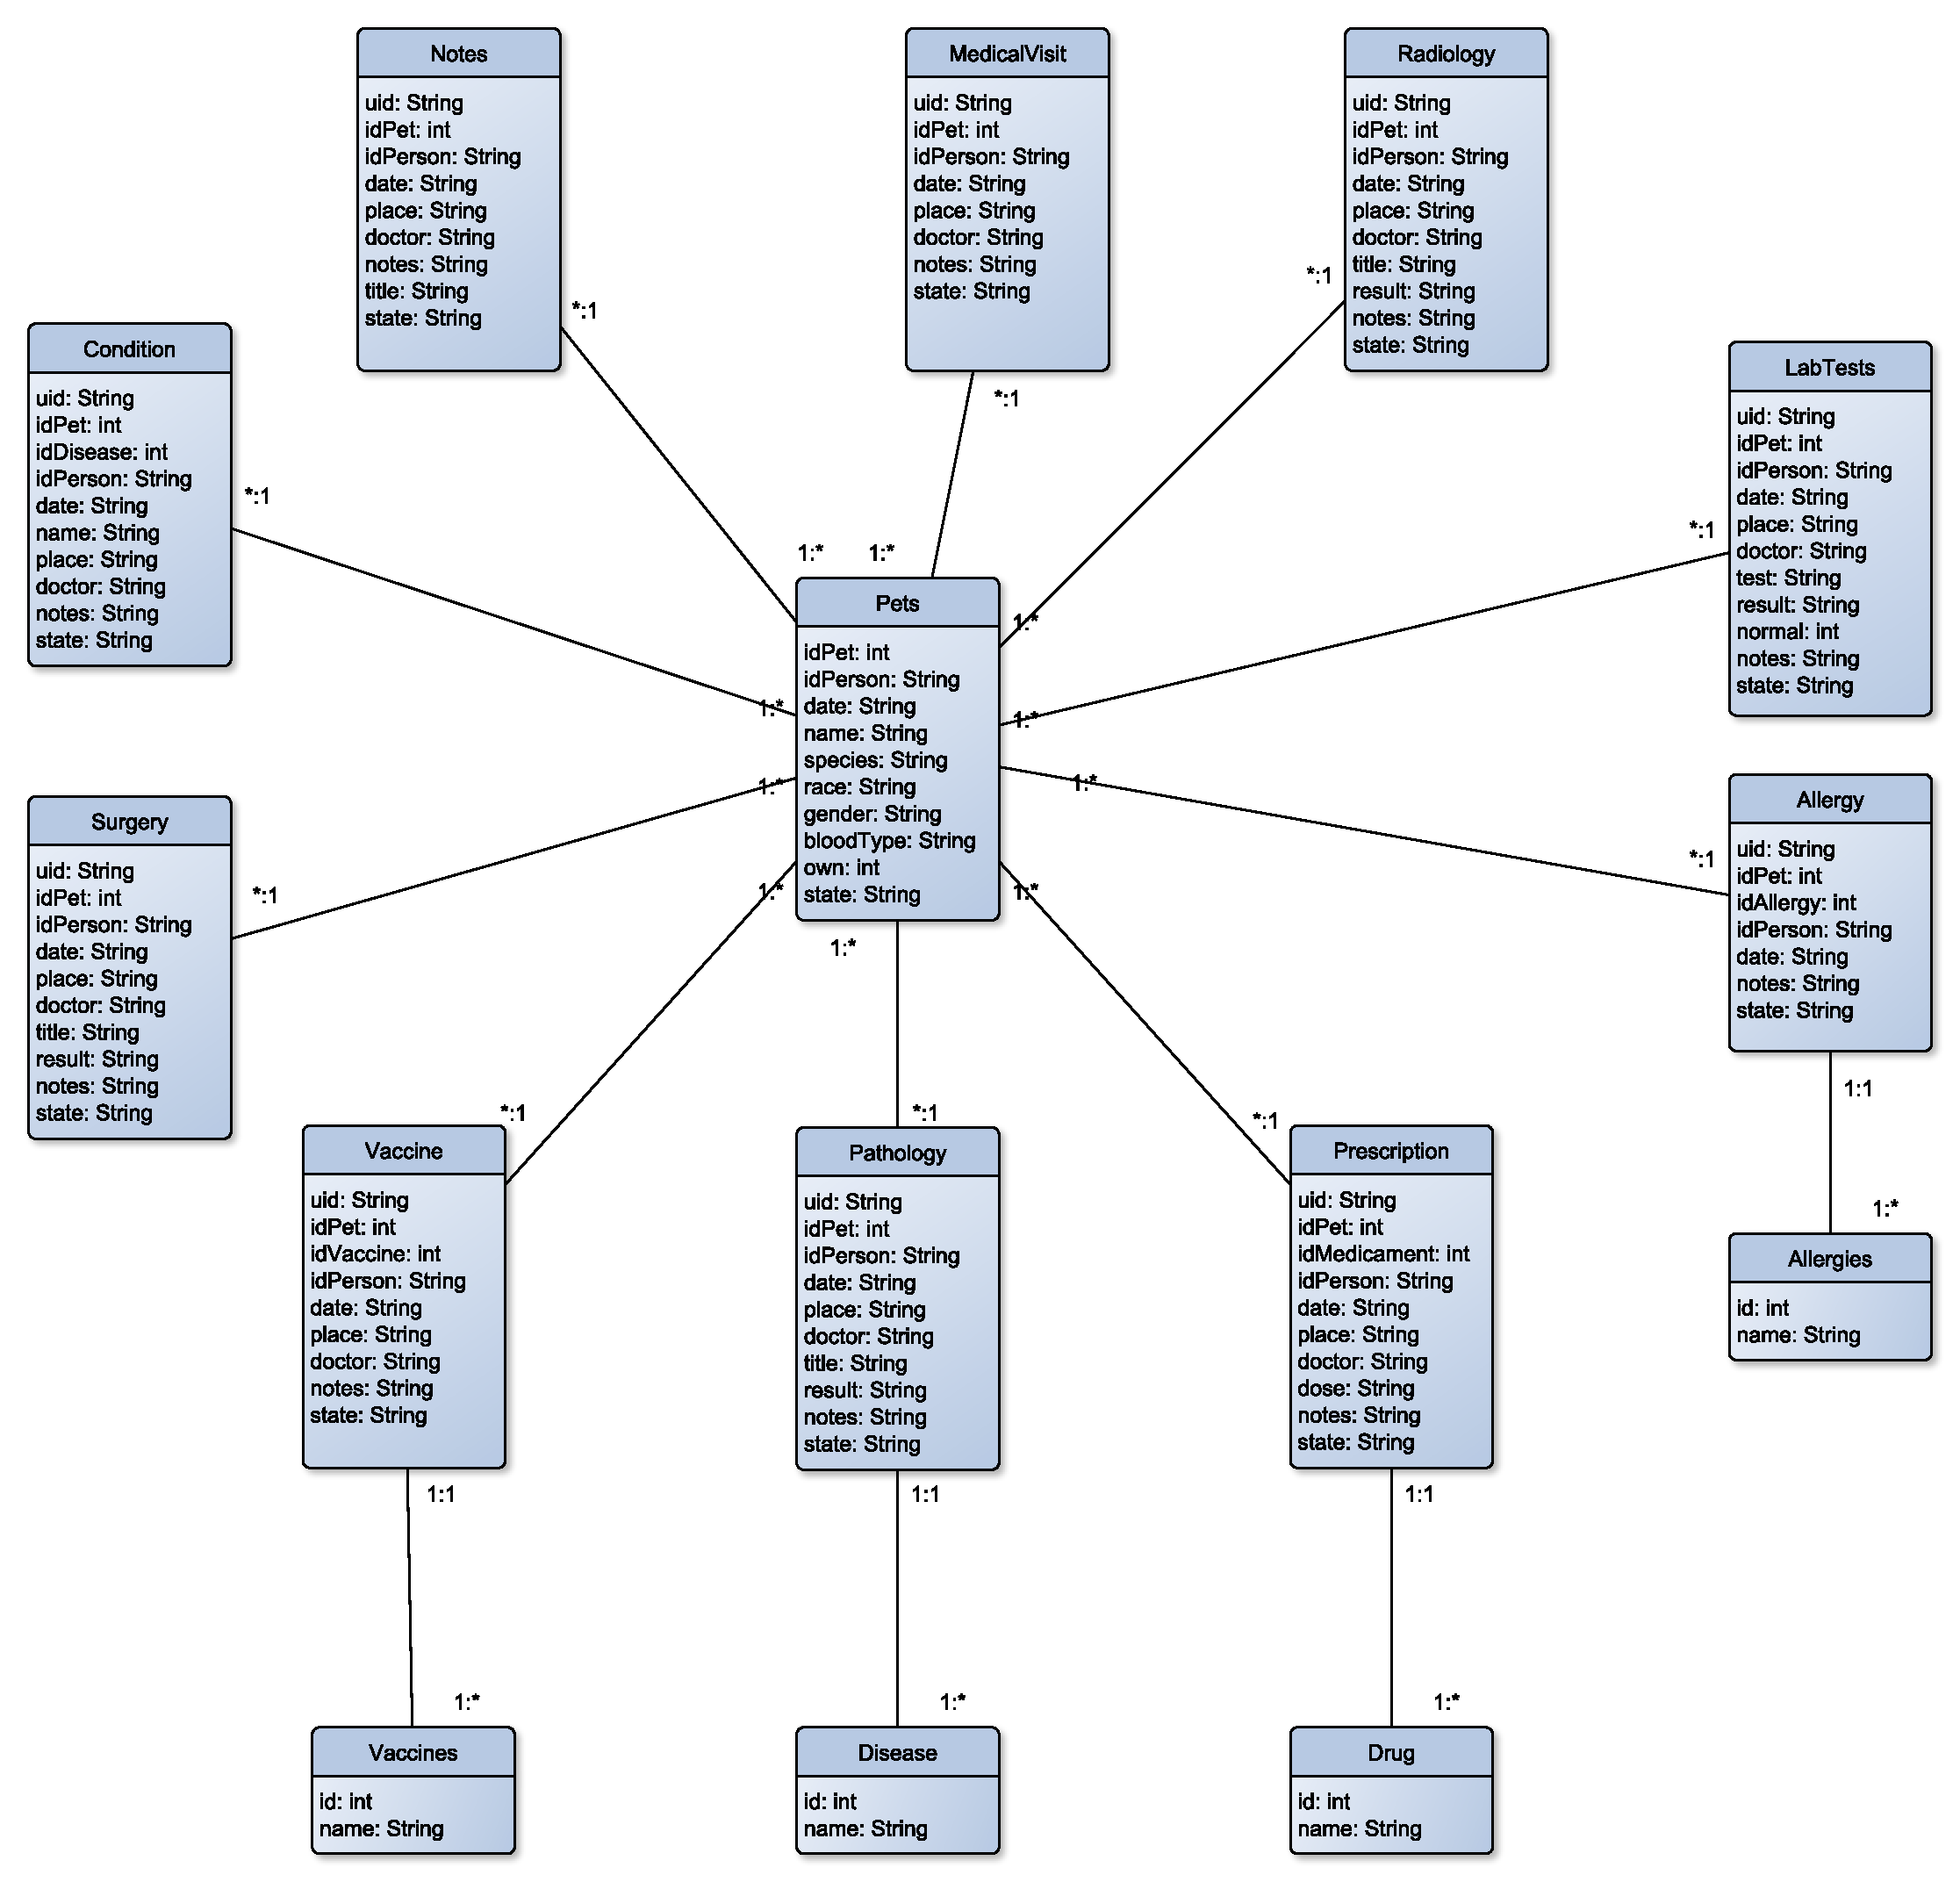
\includegraphics[scale=0.3]{Graphics/images/model1.pdf}
\caption{Representación del modelo de la base de datos}
\label{fig:rcm}

\end{center}
\end{figure}




Para la creación y acceso a la clase DatabaseHandler; clase encargada de manejar las solicitudes a la base de datos en nuestra aplicación, se utilizó como patrón de diseño singleton. 

\textbf{Singleton} \brackcite{single} es un patrón de diseño creacional que consiste en tener durante toda la ejecución de un programa sólo una única instancia de una clase dada; proveyendo además un punto de acceso global a dicha instancia. Esto se logra entre otras cosas haciendo privado el método constructor de la clase y ofreciendo acceso a esta a través de un método especial de tipo get. Dicho método es el encargado de verificar si existe creada una instancia de esa clase y devolverla o crearla dependiendo del caso. De esta forma se asegura la propia clase de haber sido creada una única vez y por tanto tener una única instancia (singleton).



\chapter{Detalles de Implementación}
\label{chapter:implementation}


\section{Tecnologías utilizadas en HCVet}


\subsection{Dart}


%\begin{figure}[h!]
%\begin{center}
%
\includegraphics[scale=0.4]{Graphics/images/LogoDart.png}
%\caption{Logo de Dart}
%\label{fig:rcm}

%\end{center}
%\end{figure}

Para la implementación de la aplicación se empleó como núcleo principal $Dart$ \brackcite{dart}. $Dart$ es un lenguaje optimizado para el desarrollo rápido de aplicaciones en cualquier plataforma, su objetivo es ofrecer el lenguaje de programación más productivo para el desarrollo multiplataforma. $Dart$ es un lenguaje orientado a objetos, basado en clases, con una sintaxis similar a $C$ y con $Garbage Collector$\footnote{Garbage Collector o Recolector de basura es un mecanismo implícito de gestión de memoria implementado en algunos lenguajes de programación de tipo interpretado o semi-interpretado.}. Admite interfaces, genericidad\footnote{Es una propiedad que permite definir una clase o función sin especificar el tipo de datos de uno o mas de sus parámetros }, mixins\footnote{Es una clase que contiene métodos para ser usados por otras clases sin tener que ser la clase padre de esas otras clases. }, clases abstractas,  e inferencia de tipos. 

$Dart$ también es la fundación de $Flutter$ proveyendo el lenguaje y los tiempos de ejecución que caracterizan a $Flutter$.

%https://dart.dev/overview


\subsection{Kotlin}

%\begin{figure}[h!]
%\begin{center}
%
\includegraphics[scale=0.11]{Graphics/images/LogoKotlin.jpg}
%\caption{Logo de Kotlin}
%\label{fig:rcm}

%\end{center}
%\end{figure}

Para la implementación de algunas funcionalidades de la aplicación se utilizó $Kotlin$ \brackcite{kot}. $Kotlin$ es el lenguaje oficial para desarrollo de aplicaciones en $Android$ declarado por $Google$ en el $2019$. $Kotlin$ es un lenguaje de programación multiplataforma que remueve detalles superfluos de $java$ como $null pointer exceptions$ \footnote{$null pointer exceptions$ es una excepción que ocurre cuando una variable es accedida en ejecución y esta no está apuntando a ningún objeto} y es un lenguaje más simple y práctico en comparación con $java$.




%https://developer.android.com/kotlin/overview
\subsection{Paquete http}

\textbf{http} es una biblioteca de $Flutter$ basada en \textbf{Future}\footnote{Una instancia de la clase \textbf{Future} representa el resultado de una operación asíncrona} para hacer \textbf{requests} de $HTTP$.

Esta biblioteca es multiplataforma que permite su uso en dispositivos de escritorio, dispositivos móviles y en navegadores web. Contiene una variedad de funciones y clases de alto nivel que facilitan el consumo de recursos $HTTP$. 

\textbf{http} \brackcite{httpF} es uno de los paquetes más aclamados de $Flutter$ que se encuentran disponible en $pub.dev$.

\subsection{Paquete uuid}
Este complemento para $Flutter$ se encarga del análisis y la generación simple y rápida de \textbf{UUID}\footnote{Identificador Único Universal}  RFC4122. Entre las posibles opciones de obtención de uuid la que se utilizó para las llaves de las tablas fue la basada en el tiempo \brackcite{uuid}. 


\subsection{Paquete encrypt}
Esta biblioteca contiene un conjunto de APIs de alto nivel sobre $PointyCastle$\footnote{$PointyCastle$ es una biblioteca de $Dart$ para encriptación y desencriptación.} para criptografía simétrica. Facilita la generación de llaves aleatorias seguras y Vectores de Inicialización.


\subsection{Paquete sqfentity}
\textbf{SQLite}\brackcite{sqli} es una biblioteca en lenguaje $C$ que implementa un motor de base de datos $SQL$ pequeño, rápido, autónomo, de alta confiabilidad y con todas las funciones. El formato de archivo que utiliza es estable, multiplataforma y compatible con versiones anteriores.
 
Entonces llegamos a \textbf{sqfentity}\brackcite{sqfen}, un $ORM$\footnote{Es una técnica de programación para convertir datos entre el sistema de tipos utilizado en un lenguaje de programación orientado a objetos y la utilización de una base de datos relacional como motor de persistencia.}  para $Flutter$ $SQLite$. Se basa en el paquete $sqflite$, para la misma plataforma, permitiendo compilar y ejecutar comandos $SQL$ de manera fácil y rápida con la ayuda de métodos fluidos similares a $Entity$ $Framework$ de $.Net$\footnote{El Entity Framework es un conjunto de tecnologías de ADO.NET que admiten el desarrollo de aplicaciones de software orientadas a datos}.

\section{Detalles de la Implementación}
\label{chapter:implementation}

\subsection{Estructura de Model}

En el Modelo de la aplicación se buscó proporcionar todas funcionalidades deseadas del producto de la forma más legible y escalable a futuro que fuera posible. Con este objetivo los autores tomaron el patrón de arquitectura de micro-servicios \brackcite{arqPat}, se dividió el modelo en 3 componentes de servicio: 

\begin{itemize}
\item Componente de comunicación con el servidor ($Online$)
\item Componente de transferencia de datos no sincronizada sin conexión a internet. ($Offline$)
\item Componente de almacenamiento interno ($Database$)
\end{itemize}

Con los componentes de servicio definidos se emplean las interfaces del $ViewModel$ para acceder a estos servicios. Consideramos que este diseño permitía crear un modelo escalable horizontalmente \footnote{El escalado horizontal refiere a la adición de componentes adicionales para hacer frente a nuevas demandas} además de facilitar el mantenimiento y actualización de dichos componentes.

\subsection{Implementación de la transferencia de datos no sincronizada}

Uno de los requerimientos fundamentales del producto era lograr la compatibilidad con la mayor cantidad de dispositivos móviles que fuera posible, intentando evitar la necesidad de adquirir un dispositivo móvil moderno para poder utilizar el producto.

Durante la investigación realizada para satisfacer este requisito los autores encontraron un problema: los paquetes de $Flutter$ encontrados que permiten el manejo las conexiones entre dispositivos a través de $Wifi$ restringían el uso de diferentes $APIs$ como la creación de $Hotspots$ locales para el $SDK$ de $Android$ mayor o igual que $26$ \footnote{$Android$ $SDK$ $26$ refiere al sistema operativo $Android$ $8.0$} \brackcite{wifiIOT}.

Para suplir esta necesidad se utilizo el $API$ $WifiP2pManager$ de $Android$. Esta $API$ permite a la aplicación descubrir $peers$\footnote{$Peer$ en un contexto de $network$ es un nodo que cumple la misma funcionalidad que otro nodo en la red. Cualquier usuario que se conecta a la red de intercambio es un $peer$} disponibles y permite establecer una conexión directa con estos. Usando $Kotlin$ se definió el comportamiento de los $peers$ y se creó una interfaz para acceder a las funcionalidades de esta $API$.

\subsubsection{¿Cómo se usa esta interfaz desde $Flutter$?}


$Flutter$ permite realizar llamados a $APIs$ específicas de la plataforma disponibles en $Java$ o $Kotlin$ en $Android$ y en $Objective$ $C$ o $Swift$ en $iOS$

Desde la aplicación de $Flutter$ se envía un mensaje a un $host$ en $Android$ o $iOS$ a través de un canal entre plataformas. Tanto el mensaje como la respuesta se pasan de forma asíncrona.

\subsection{Implementación del componente Online}
La comunicación con el servidor está basada en un protocolo de tipo $Hypertext$ $transfer$ $protocol$ $secure$ ($HTTPS$) de $request-response$. Se consideró la encriptación de los datos en ambas direcciones que ofrece el protocolo $https$ para evitar la vulneración de datos sensibles transferidos como pueden ser el $id$ del usuario o la mascota, correo y contraseña.

\subsection{Sincronización de la base de datos local con el servidor}
Dentro de las problemáticas encontradas durante el proceso de sincronización de la base de datos local con la del servidor se pudieran mencionar las siguientes:
\begin{enumerate}

\item\textbf{Diferenciar los datos}: en cualquier momento dado en la base de datos local existirán datos que ya el servidor tendrá conocimiento de ellos y por tanto se puede decir que están sincronizados con el servidor y otros datos de nueva creación que hasta que no exista una conexión a internet, el servidor desconocerá por completo de su existencia y por tanto estarán pendientes a sincronizar. Diferenciar cuales de estos datos ya están sincronizados y cuales no, resulta un poco complejo de manejar si no se utiliza algún mecanismo de “control” sobre ellos. Todo esto para intentar reducir el número de envío de información al servidor por cuestiones de seguridad y rapidez, puesto que bien se podrían enviar todos los datos de la base de datos local al servidor cada vez que exista una conexión, pero esta opción además de no factible resulta lamentable. Para solucionar dicha problemática se optó por agregar en cada tabla de la base de datos un campo extra llamado “$state$”. Dicho campo tendrá el valor “$waiting$” cuando es un dato nuevo y el valor “$synchro$” cuando ya ha sido sincronizado con el servidor. Cuando los datos son creados desde el propio teléfono la función de insertar elementos en la base de datos declara el campo $state$ de dicho objeto como $waiting$, sin embargo, cuando los datos provienen de otro móvil o incluso del propio servidor se declara el $state$ como $synchro$ puesto que no es necesario re sincronizar  estos datos.
\item\textbf{Guardar llaves de futuras mascotas}: cuando el usuario se registra en el servidor y/o realiza algún tipo de suscripción, el servidor manda una lista de futuras llaves para la creación de nuevas mascotas. Para no tener que implementar una nueva tabla que tan solo guardase estas llaves o bien almacenarlas en un fichero apartado de la base de datos, se optó por almacenar en la tabla $Pets$ una mascota “vacía”. Dicha mascota tendrá en sus campos solo esta llave como llave primaria y el $state$ tendrá el valor “$empty$” indicando de este modo que la mascota aun no existe en la base de datos. Cuando se crea una nueva mascota que tiene alguna de estas llaves como llave primaria se actualizan los campos de la mascota ya “previamente” insertada en la base de datos y su $state$ cambia a “$waiting$”.
\item\textbf{Guardar mascotas eliminadas}: aunque pareciese una contradicción hay momentos en la que nuestra base de datos necesita mantener guardada aun una mascota que ha sido eliminada por el usuario. Como nuestra base de datos debe ser sincronizada con la existente en el servidor no basta con eliminar una mascota directamente de la base de datos cuando el usuario requiera esta operación puesto que, si la mascota deja de existir, luego cuando exista una conexión a internet no habrá manera de indicar al servidor que debe eliminar dicha mascota de su base de datos también. Para resolver esta problemática se hace uso nuevamente del campo $state$ en mascota. Cuando el usuario manda a eliminar una mascota de la aplicación, se actualiza el $state$ de dicha mascota a valor “$delete$” indicando así al resto de los métodos de la base de datos que esa mascota, aunque está insertada no cuenta como una mascota válida (este funcionamiento se extiende también a todas las tablas que tienen como llave foránea un id de dicha mascota). Luego de que se indique al servidor que debe eliminar dicha mascota se eliminará también de la base de datos local.
\end{enumerate}

\chapter{Pruebas de Funcionalidad y Experimentos}

En este capítulo se realizan un conjunto de pruebas para demostrar el funcionamiento de las herramientas implementadas en la aplicación.

Las pruebas fueron realizadas en dos teléfonos $android$ con las siguientes características.

Primer teléfono:

\begin{itemize}
\item Procesador: Hisilicon Kirin $710F$.
\item 4 $GB$ de $RAM$.
\item Sistema Operativo Android $9$
\end{itemize} 

Segundo teléfono:

\begin{itemize}
\item Procesador: Octa-core Max $2.00GHz$.
\item 4 $GB$ de $RAM$.
\item Sistema Operativo Android $12$
\end{itemize} 

\newpage
\section{Prueba 1: Creación de cuenta o autentificación de usuario}

\begin{figure}[h!]
\begin{center}

\includegraphics[scale=0.25]{Graphics/images/hcvet/init.jpg}
\caption{De izquierda a derecha: Página inicial de la aplicación, página de creacióm de usuario y página de autentificación}
\label{fig:bac}

\end{center}
\end{figure}

Se requiere que el usuario introduzca un nombre de usuario y contraseña para crear una cuenta en el servidor. La aplicación también utiliza el número de teléfono del dispositivo para identificar al usuario. En caso de que el número de teléfono o el correo introducido ya se encuentre registrado la aplicación muestra un error y espera una corrección por parte del usuario.

\newpage
 
\section{Prueba 2: Creación de mascota}

\begin{figure}[h!]
\begin{center}
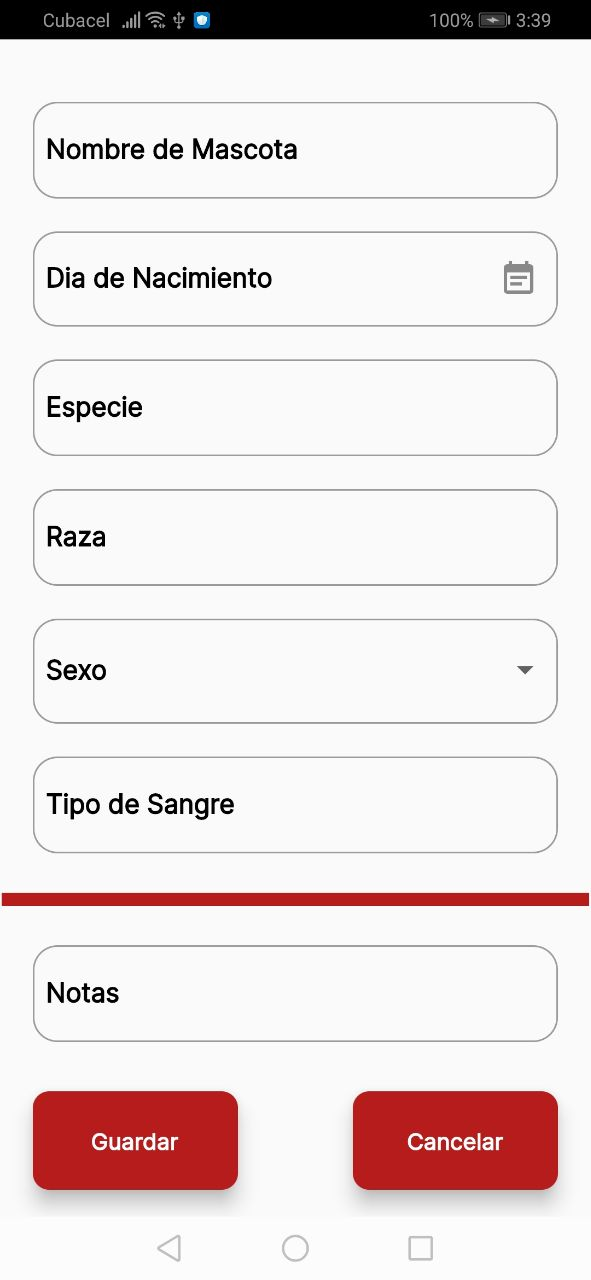
\includegraphics[scale=0.15]{Graphics/images/hcvet/addpet.jpg}
\caption{ Página de creación de mascotas}
\label{fig:bac}

\end{center}
\end{figure}

La creación de una mascota requiere que el usuario introduzca todos los campos que se listan a excepción de $notas$. Solo se permite la creación de una mascota si el usuario tiene un $id$ disponible en la base de datos local.

\begin{figure}[h!]
\begin{center}
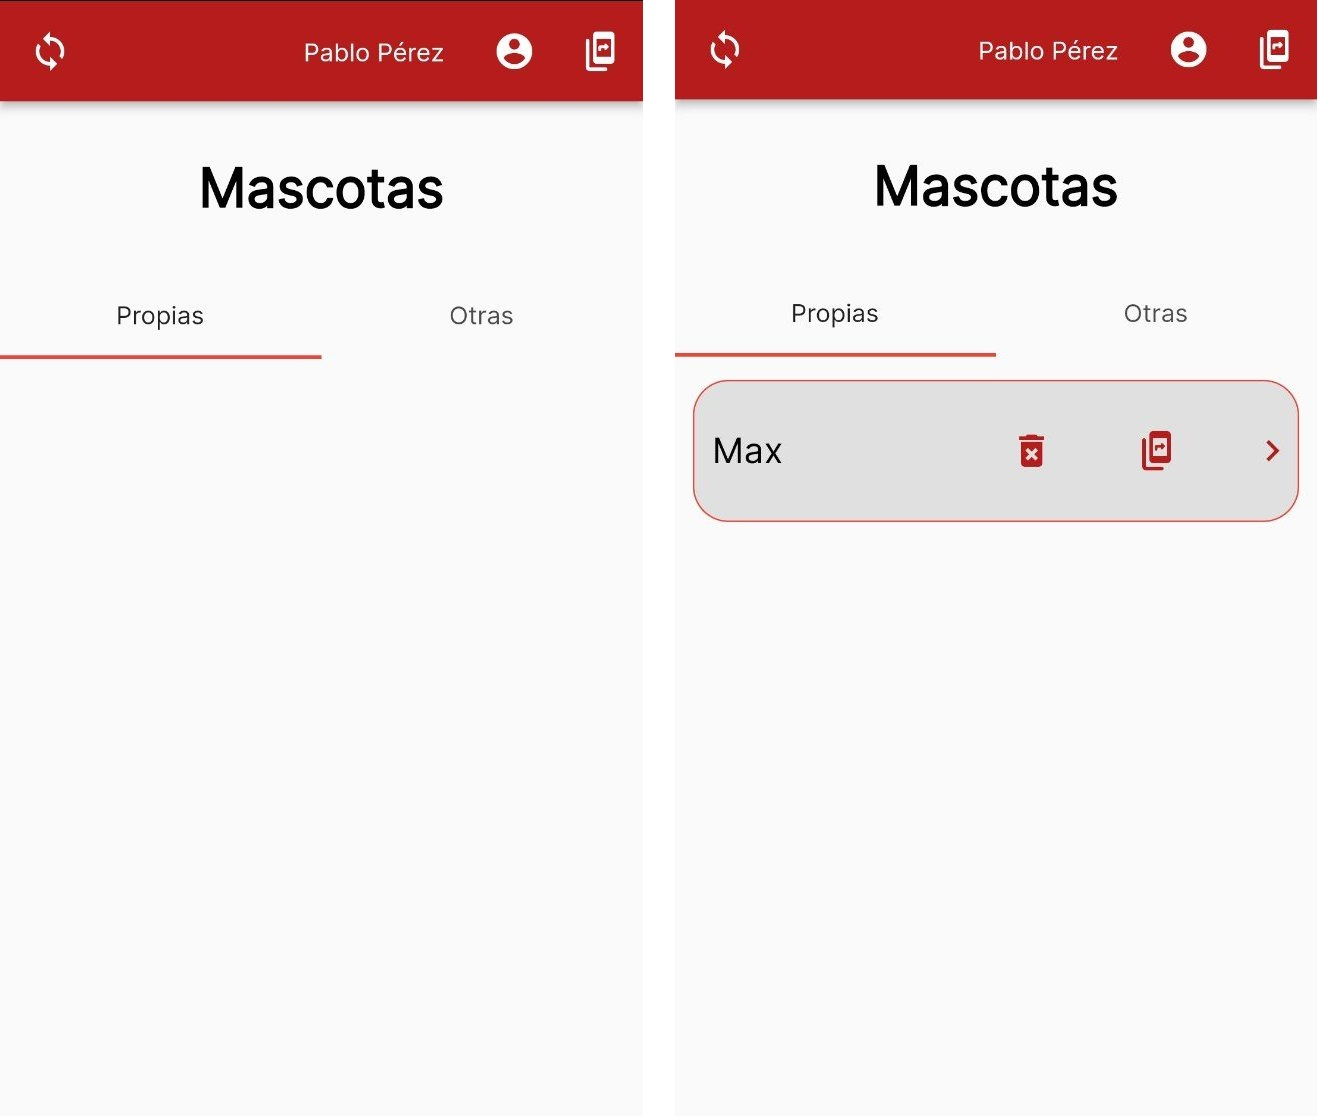
\includegraphics[scale=0.19]{Graphics/images/hcvet/home.jpg}
\caption{ Página de central de la aplicación antes y después de crear una mascota}
\label{fig:bac}

\end{center}
\end{figure}

Página central de la aplicación antes y después de crear una mascota

\newpage
\section{Prueba 3: Eliminar mascota}

\begin{figure}[h!]
\begin{center}
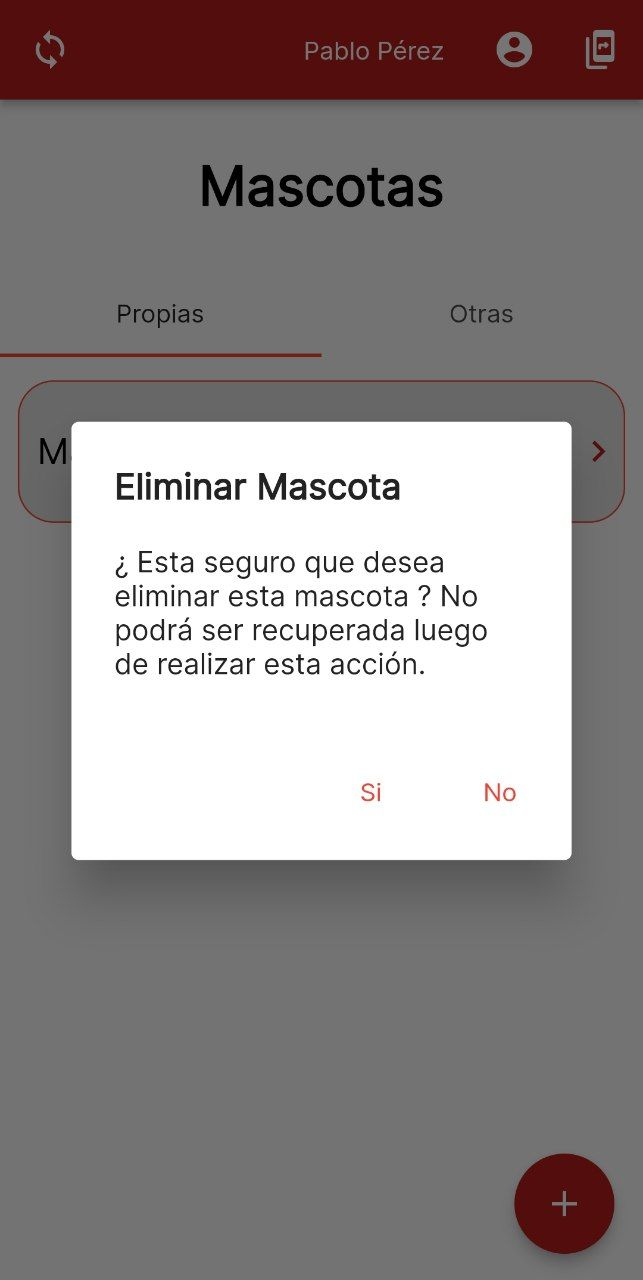
\includegraphics[scale=0.19]{Graphics/images/hcvet/delete.jpg}
\caption{ Advertencia al eliminar una mascota}
\label{fig:bac}

\end{center}
\end{figure}

Si el usuario decide eliminar una mascota los datos e historial de consultas de estas no podrán ser recuperados. Esta advertencia es mostrada ante el usuario, si escoge eliminar la mascota el servidor será notificado de esta decisión la próxima vez que se sincronice.


\newpage

\section{Prueba 4: Creación y mostrado de consultas}


\begin{figure}[h!]
\begin{center}
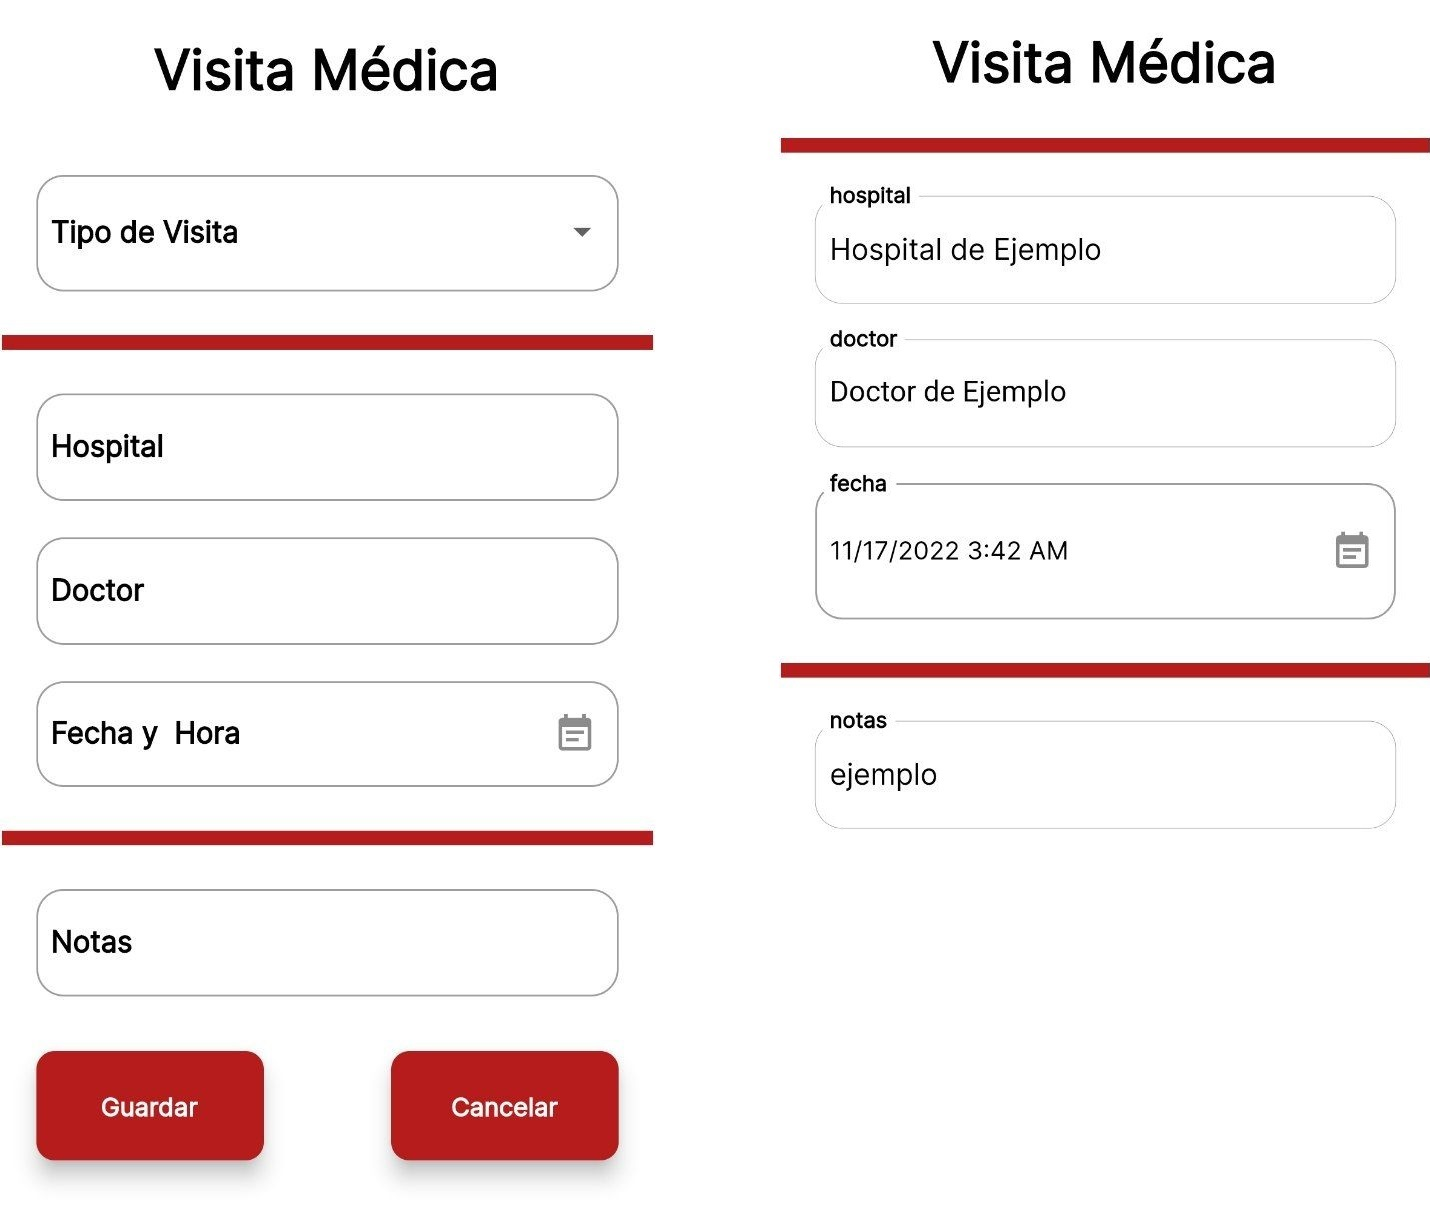
\includegraphics[scale=0.15]{Graphics/images/hcvet/medvisit.jpg}
\caption{Página de creación de consulta Visita Médica y página de mostrado de esta consulta}
\label{fig:bac}

\end{center}
\end{figure}

La creación de una consulta solo requiere un dato fundamental, la fecha. Las consultas de Prescripción, Vacuna, Condición y Alergia requieren que se seleccione una de las llaves foráneas de la respectiva consulta. El usuario es notificado si uno de estos requerimientos no se cumple.

\begin{figure}[h!]
\begin{center}
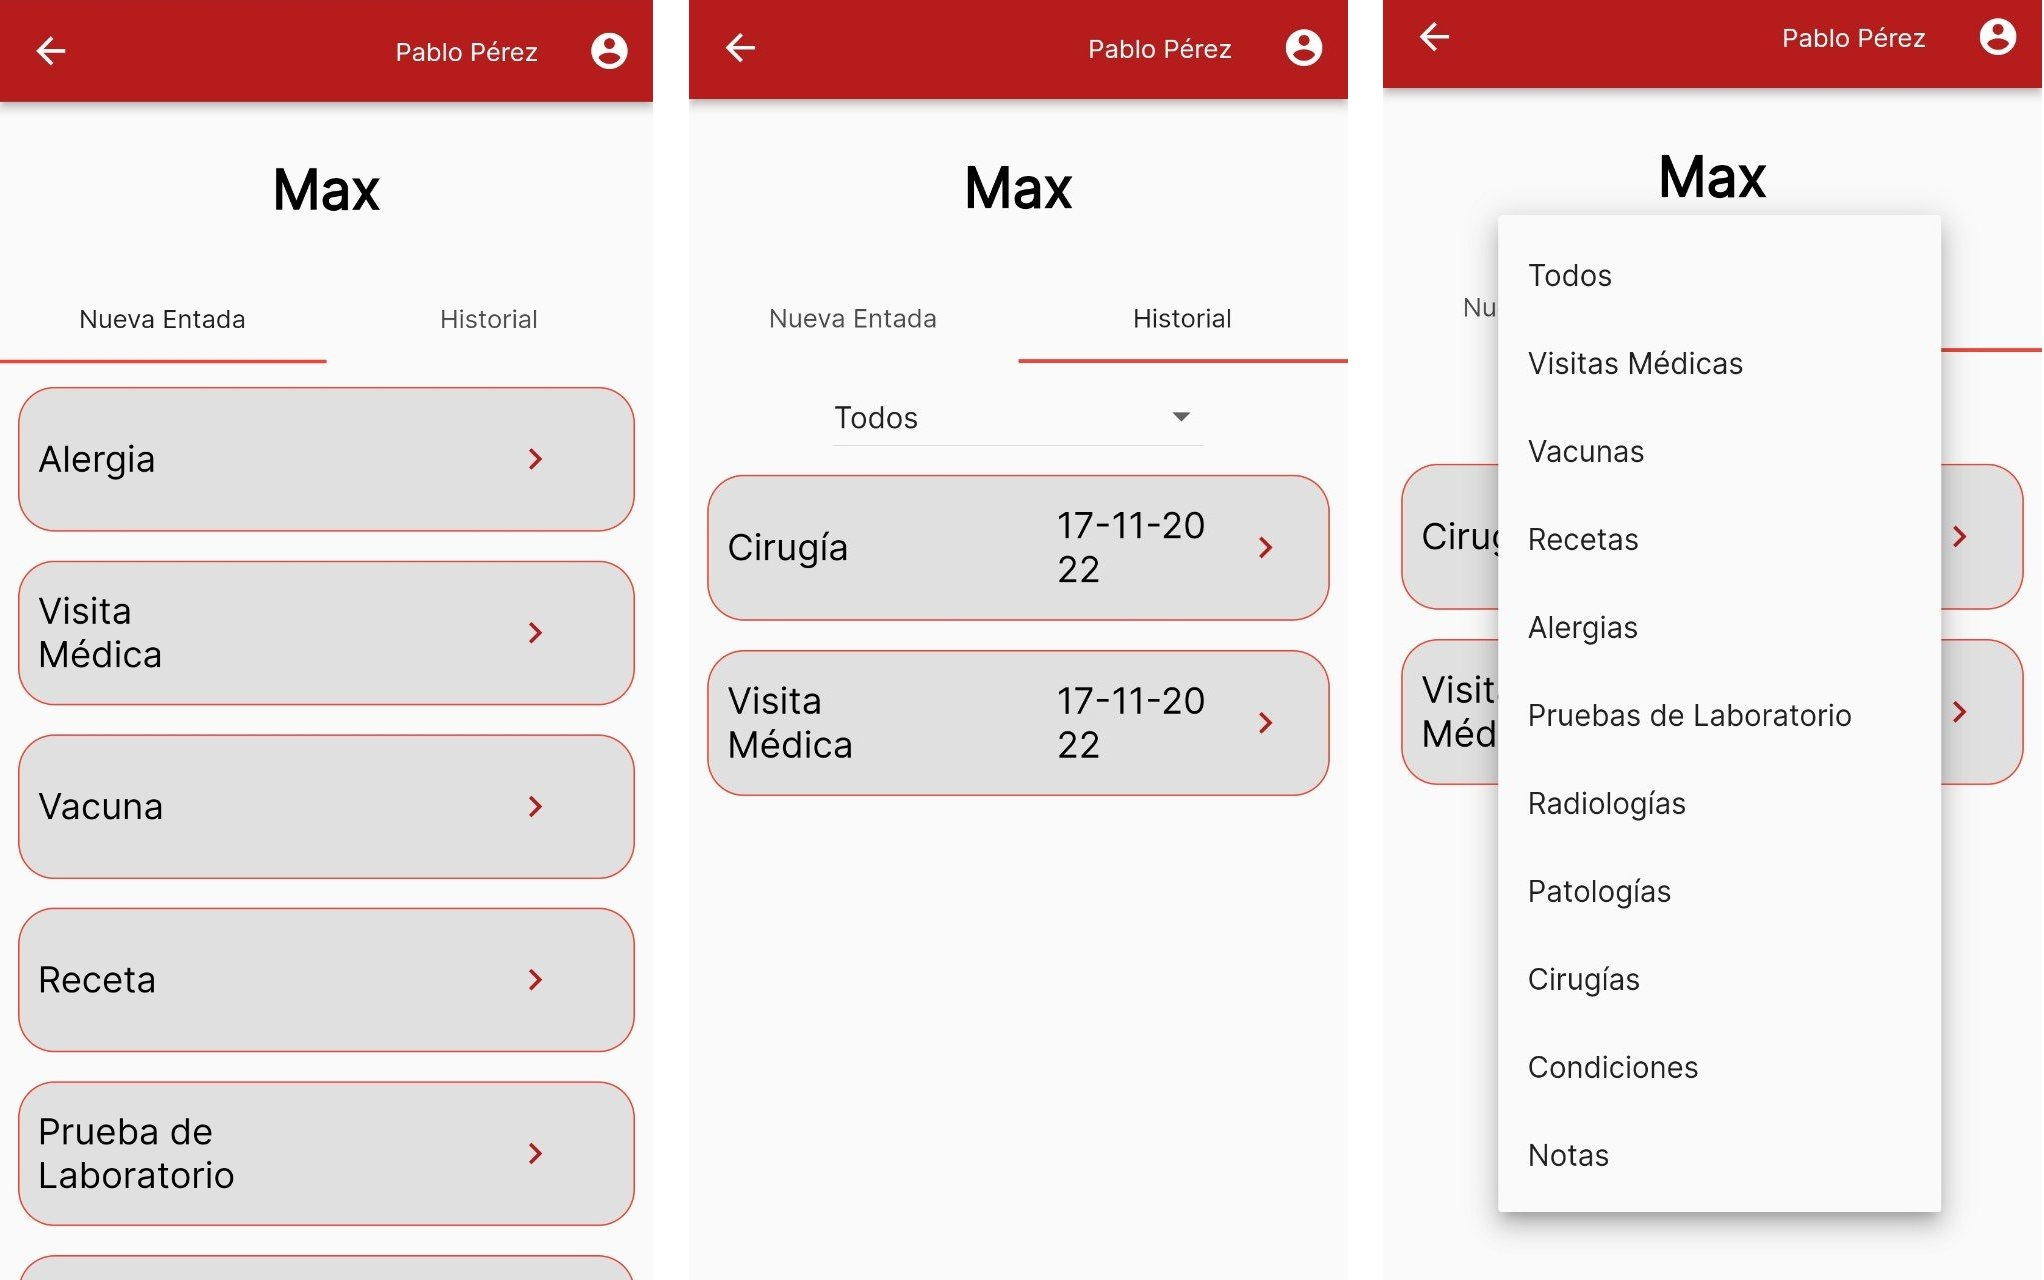
\includegraphics[scale=0.17]{Graphics/images/hcvet/formsmake.jpg}
\label{fig:bac}
\caption{De izquierda a derecha: Página de selección de consulta a agregar, historial de consultas y filtrado de consultas en historial}
\end{center}
\end{figure}

Con una mascota seleccionada se dirige al usuario a la página de manejo de consultas, el usuario puede crear una consulta nueva o acceder a todas las consultas que se encuentran almacenadas en la base de datos local.